\section{Introduction}
From 2010 to 2020 the amount of data that was processed rose from 1.2 trillion gigabytes to 59 trillion gigabytes - an increase by 5,000\% \citep{data}. This exponential growth has evoked a high demand to leverage these amounts of data to promote scientific discoveries. In particular, it motivated the use of machine learning across all disciplines. Machine learning (ML) refers to a field of study that gives computers the ability to learn without being explicitly programmed. The benefits of this approach are immediate, since it allows computational systems to automatically process and reason about the enormous amounts of data, exceeding task-specific human capabilities considerably. 
Most recently, deep learning (DL) has emerged as a sub-discipline of machine learning denoting the use of multiple hidden layers in a network. Deep learning models can achieve even better accuracy than standard machine learning architectures given the availability of a substantially greater amount of data.

A great potential of these developments in drug discovery lies within early stages to predict structure-activity relationships (SARs) and structure-property relationships (SPRs). These are grounded on the fundamental assumption that structurally similar molecules have similar activities/properties. For instance, after finding a hit compound in a drug screening campaign researchers would like to understand how its chemical structure can be optimised in order to improve properties like binding affinity, biological responses or physiochemical properties \citep{LO20181538}. Classically, this problem could only be solved through resource-intensive \emph{in vitro} screeening and \emph{in vivo} testing. Early quantitative structure-activity/property relationships (QSAR) models \citep{hansch}, that attempted to solve this problem \emph{in silico}, were limited by a lack of experimental data and the linearity assumption made for modeling \citep{LO20181538}.
The introduction of high-throughput screening (HTS) and combinatorial synthesis resulted in a rapid explosion of the availability of data screening 100,000s or more samples per day for a desired biological activity. Ultimately, this led to the development of large databases containing the profiles of millions of chemical substances. How to effectively use these amounts of data for machine and deep learning methods has become a crucial challenge for drug discovery.

In abstract terms, fitting a QSAR/QSPR model amounts to finding a generally non-linear function between a class of molecules and a desired biological activity/property. ML/DL methods solve this problem by learning this function automatically. Pretty much any machine learning methods has been applied in this second step \cite{SHEN201929} and popular examples include support vector machines \cite{supv1, supv2}, extreme gradient boosting \cite{XG1, XG2} and random forest \cite{RF1}. However, the performance of these methods crucially depends on the used mathematical representation of molecules, since it needs to describe the attributes of the molecules necessary to predict the activity/property of concern. Two approaches to design these `features' have been introduced. On the one hand, fixed representations, like descriptors and fingerprints, map a molecule to a predefined vector space that contains the numerical values of some selected properties of a molecule. The drawback of this approach is that expert knowledge is necessary in order to make a meaningful selection of properties that are useful for learning the relationship to the target activity/property. Furthermore, this selection is inherently biased by the domain knowledge \citep{merkwirth}. The other, recently emerged, class of representations is given by learned representations. Instead of manually employing a mapping to a fixed space, Recurrent Neural Networks (RNNs) and Graph Neural Networks (GNNs) can be used to learn the space itself such that is contains the most suitable properties for predicting the target values.  The typical workflow of designing features and predicting an activity/property is summarised in figure \ref{fig:mpp_workflow}.
\begin{figure}[h]
	\centering 
	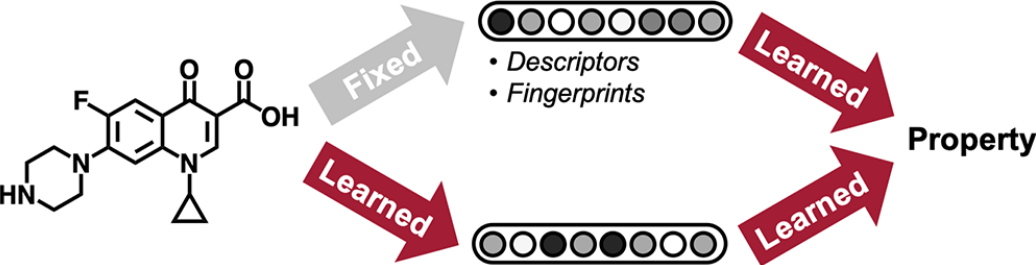
\includegraphics[width=0.6\textwidth]{MPP_workflow.png}
	\caption{Illustration of the QSAR/SQPR workflow using ML/DL. Reprinted from \cite{yangMPP}. }
	\label{fig:mpp_workflow}
\end{figure}

There are numerous examples highlighting the potential of learned representations \citep{duvenaud2015convolutional, li2019deepchemstable, honda}. Most prominently, \cite{STOKES2020688} achieved a breakthrough in antibiotic discovery when they discovered a new broad-spectrum bactericidal antibiotic `halicin' after decades of stagnation in the field. They employed a directed-message passing neural network \cite{yangMPP} at two stages of their work. Firstly, this graph neural network was used to predict growth inhibitory effects against E. Coli. Later, another D-MPNN was used to predict the toxicity of potential candidates. This finding underlines both the potential of learned representations to lead to meaningful discoveries as well as their versatility to be employed at various stages of an early-stage drug discovery workflow. 

The goal of this thesis is to present both fixed and learned molecular representations to understand the advantages and drawbacks of either approach. In the following two sections these are introduced, accompanied by technical background information where needed. Consecutively, we exemplify the application of a learned representation using the paper of \cite{STOKES2020688}. Finally, we discuss both approaches in terms of interpretability, computational costs and accuracy.  



The advancements of these methods are further motivated by the enormous costs time and costs connected to drug development. Discovery and development of a new drug can take 5000-10000 compounds to screen and 12-15 years to end up with one approved drug requiring costs of more than \$1.3B. Only 2 out of 10 approved and marketed drugs can recover these costs \cite{hecht}.`

 \begin{comment}

\section{Intro}\label{sec:introduction}

Molecules form the smallest identifiable parts of covalent compounds that still retain their chemical properties \cite{molecules}. These covalent compounds can be found in all organisms, since together they form integral parts like proteins or the DNA making an understanding of molecules and their properties key to deciphering the foundations of life. Since molecules are complex physical entities in 3D space consisting of covalent bonds between atoms, identifying their chemical, physical or biological properties is by no means a simple task. \emph{Molecular property prediction} aims to characterise molecules according to their properties. In abstract terms this amounts to finding a nonlinear function from a class of molecules to a set of predefined properties.  Classically, \emph{in vitro} screeening and \emph{in vivo} testing were widely used in early stages of drug discovery in order to identify 'druggable' targets that display a desired biological response. Lead compounds were found by isolating natural products from microbiological fermentation, plant extracts and animal sources \cite{Gallop1994ApplicationsOC}. However, this process is extremely time and resource inefficient, because ... . More recently, \emph{in silico} methods attempt to embed the molecule into a mathematical representation which can then be used to learn this nonlinear relationship between the embedded molecules and their corresponding properties using statistical and machine learning methods. For instance, J. Stokes et al. achieved a huge breakthrough when the discovered the new antibiotics halicin \cite{STOKES2020688} after decades of stagnation in that field. Contrary to previous methods that translate molecules into a fixed predefined mathematical representation, they employed a Graph Neural Network that was able to learn a representation that then served as an input to an Artificial Neural Network to predict the target inhibitory effect against E. coli. %TODO: double check
Other classes of properties that have been of interest in the past are vast and comprise for example quantum-mechanic, physio-chemical, bio-physical or physiological properties \cite{wu2018moleculenet}. 

On October 5, 1981 a new version of the 'Fortune' magazine was release. Its cover page featured an article titled 'The   Next Industrial  Revolution:  designing  drugs  by  computer  at Merck' \cite{article}. This marked the begin of stage of naive euphoria in computational drug design with investments of millions of dollars in hardware and software. 
\subsection{Outline of the thesis}
The goal of this thesis is to investigate the role of Graph Neural Networks in the field of Molecular Property Prediction and its application to Drug Discovery being one of its best known representations in biology. In the rest of this section we will give a brief outline of the history of the dominant methods in MPP and elaborate on its role in Drug Discovery. Following that, we will introduce Graph Neural Networks and present the necessary theory behind them in order to understand their advantages and disadvantages. Then, we will compare the performance of GNNs to that of other methods in MPP and assess the benefit of Deep Learning in MPP in general. Finally, a summary of this thesis is given outlining its most important findings. 
\subsection{Disclaimer}
High level approach. Mathematically rigorous descirption can e found in \cite{KerberAdalbert2014Mcac}.




\subsection{Molecules}
Atoms are the smallest identifiable units of chemical elements which make up all matter in the universe. A fundamental principle of chemistry is that the atoms of different elements can combine to form chemical compounds and a lot of the study in chemistry is centered around understanding what happens when these compounds are formed. A chemical compound can be defined as a distinct group of atoms that are held together by chemical bonds (cite? Khan modelcules). Similar to the attraction between the positively charged nucleus and the negatively charged electrons that constitutes the structure of atoms, chemical bonds are caused by electrostatic attractions. While there is no clear separation between types of bonding from a physical perspective, it is still convenient to distinguish between different bonding types from a chemical perspective. The behaviour of the valence electron is the determining factor and this can be responsible for different properties of the resulting substance.

We are primarily concerned with two major types of bonds: Ionic bonds and covalent bonds.
In a simplified view, ionic bonding can be classified  as the transfer of a valence electron from one atom to the other resulting in the formation of two oppositely charged ions that hence attract each other and are bond together. Covalent bonding on the other hand is the result of electrostatic attraction between one or more electrons to the atomic nuclei of both atoms. This can be regarded as a sharing of the electrons across the two atoms. The structure resulting from covalent bonding is called a \emph{molecule}. These are of particular importance in biology making up the smallest identifiable parts of \emph{covalent compounds} that still retain their chemical properties \cite{molecules}. These covalent compounds can be found in all organisms, since together they form integral parts like proteins or the DNA making an understanding of molecules and their properties key to deciphering the foundations of life.


\subsection{Brief history of molecular representations}
In 1860 when the first International Chemical Congress was held in Karlsruhe, Germany, Alexander Butlerov predicted that determining the atomic arrangements of molecules would be the future of chemistry \citep{butlerov1861einiges}. He was the first person to use the word `structure' in its modern chemical meaning. This marked the birth of structural chemistry.\citep{wiswesser1968107}. Since then it took only seven year to develop the main ideas about line-formula conventions in familiar form like $$\chem{C_3H_7OH}.$$
No new practices appeared within 79 years until between 1947 and 1954 structure-delineating notations were introduced such as the Wiswesser line notation (WLN) which became very popular as it was easily interpretable by humans as well as computers. Compared to today's line formulae the WLN was very compact since memory efficiency was a critical factor in computers at that time.

When the advent of technology in the science accelerated in the 1980s, the role of chemical notations began do decline. \citep{Lawlor} attributes this to two main reasons. On the one hand, computer-manageable connection tables opened up new possibilities to experiment with structures. This meant that rather than working with the chemical formula itself, it was translated in a connection table where algorithms like similarity searches could be run to calculate compute properties, map reactions etc. 
The second reason is the increasing availability of graphics terminals. Multiple companies like Molecular Design Ltd. or CAS \citep{cas} introduced interactive services that enabled a translation between a graphical representation of compounds and their connections tables. Furthermore, this involved functionalities like searching by structure or substructure diagrams, which allowed chemists to perform the searching by themselves rather than being dependent on their information scientist intermediaries. Thus, a lot of popular representations that are still used today have shifted from prioritising their compactness to being specifically designed for computer applications \citep{smiles, heller2015inchi, cereto2015molecular}. Most prominently, the SMILES (Simplified Input Line Entry System) representation \citep{smiles} assigns a molecule a string of characters, where atoms are encoded by their atomic symbol and bonds are depicted by one of the following symbols: (-, =, \#, *, .). Furthermore, branches, rings and charge can be represented by the use of brackets numbers signs (+, -) making SMILES a versatile linear notation that is used to date. 

Nowadays, the use of molecular representations has branched. On the one hand, atom based representations like SMILES or InCHi are still present in chemical databases in order to uniquely identify a given molecule in a convenient language. These can be used in order to rebuild the molecule based on the representation \cite{molrep}. On the other hand, the advent of machine learning methods in all application domains demands a numerical representation of a molecule that represent its properties. Therefore another branch of representations is given descriptors that encode structural or chemical properties. Two established classes of descriptors are decsribed in detail  in section \ref{sec:fixed_rep}. 

 the reigning paradigm in molecular representations is given by fingerprint vectors, first introduced in , and descriptors. These methods have been experiencing particular popularity, because these representation can easily be used as the input for machine learning techniques for property prediction. However, this paradigm slowly begins to be challenged by newly emerging deep learning techniques such as Graph Neural Networks.
Rather than assigning molecules a fixed representation, these techniques aim to learn  that works.a flexible representation depending on the properties of interests of the molecules. This new approach seems equally innovative as crazy (TODO different word) and we will discuss the prospects of this in the following. 
\end{comment}
\section{Fixed Representations}
\label{sec:fixed_rep}
Mapping molecules to a fixed representation is the classical form of generating a machine-interpretable input for QSAR/QSPR models. As the name suggests these are characterised by a fixed target space that contains a pre-selected choice of local or global information about the molecule.  Fixed representations can be broadly separated into two categories: Molecular descriptors and fingerprints. Descriptors are generally characterised by a more holistic representation of the molecule. Fingerprints, on the other hand, are local in nature by aggregating information of subgroups of atoms in a molecule.

\subsection{Descriptors}
According to \cite{todeschini2008handbook} `The molecular descriptor is the final result of a logical and mathematical procedure which transforms chemical information encoded within a symbolic representation of a molecule into an useful number or the result of some standardized experiment'. This definition highlights the purpose of a descriptor to generate a numerical representation, such as a vector of numbers, from a symbolic representation.

The expectations for the usefulness of a descriptor vary a lot depending on the application domain but according to \cite{Mauri2016} these typically include
\begin{enumerate}
	\item invariance to node reorderings,
	\item invariance to rotations and translations of the molecule,
	\item definition by an umabiguous algorithm,
	\item well-defined applicability to molecular structures.
\end{enumerate}
These desiderata are supposed to guarantee that the descriptor always gives the same representations for molecules that are considered the same and is generally applicable to all molecules. Beyond that, common extra requirements concern the inclusion of structural information (according to the fundamental principle of chemistry that different structures possess differeny properties), certain discriminative abilities and degeneracy/continuity, i.e. small structural differences result in small but existing differences in the value of the descriptor. 

The variety of different descriptors that have been used for QSAR analysis is enormous and depends highly on the considered application.
Any attempt to group descriptors into different categories would be quite arbitrary given the sheer amount of different application domains and descriptors. However, \cite{descript} propose an grouping based on the nature of the structural information that they require: Constitutional, topological, geometric and quantum mechanical descriptors. 

.

Constitutional descriptors are the most rudimentary form of descriptors as they do not take into account any spatial information about the molecule but just its basic structural properties. Examples include basic attributes like the molecular weight the number of atoms but also more complex ones such as the sum of atomic van der Waals volumes. 

Topological descriptors are based on the connectivity of the atoms in a molecule and encode 2D structural properties using graph invariants of the underlying molecular graphs, i.e. properties that only depend on the abstract mathematical object and not on a particular labeling or ordering of the vertices. Such invariants include the Wiener index \cite{wiener1947structural, nikolic2001wiener} $W = \frac{1}{2} \sum_{i,j}^ N d_{ij}$, where $N$ is the number of non-hydrogen atoms and $d_{ij}$ is the edge count of the shortest part between atoms $i$ and $j$. A drawback of topological descriptors compared with constitutional descriptors is that they often tend to be less interpretable due to the abstract nature of the underlying graph. 

Geometric descriptors receive 3D information about the molecule as their input which may be resourceful to obtain from crystallographic data or molecular optimization \cite{Mauri2016}. However, they may also come with more information compared to descriptors that receive lower dimensional inputs. Therefore, they are usually employed in domains when this additional information is critical such as when two conformations are compared (TODO rewrite). An example of a geometric descriptor is given by the 3D Wiener Index which extends the 2D case by weighing the edges by their actual length or the gravitation index \cite{katritzky1996correlation}.

Finally, quantum mechanical descriptors are based on quantum mechanical calculations. For instance, they have been used to predict toxicity of molecules in QSAR studies \citep{REENU201589, senior2011qstr}. However, their tendency to require high computational costs impediment their application ot large scale virtual screenings.

Note that these categories are a non-exhaustive classification of descriptors and many others exist such as auto-correlation descriptors \citep{broto1984molecular} (TODO one more?). We conclude that descriptors are a popular method to represent molecules as they are a flexible means to encode the properties that are relevant to the particular application domain. However, this comes also with a downside as the performance of the application may heavily depend on the choice of descriptors and this selection is by no means a trivial task.

\subsection{Fingerprint Vectors}

All descriptors considered so far are derived from performing mathematical computations on the underlying structure and give a holistic representation of the substances considered. Fingerprint vectors on the other hand are given as bit vectors that indicate the presence or absence of a local property and are thus local in nature. Two classes of fingerprints can be distinguished \citep{SHEN201929}: Dictionary-based and hash-based fingerprints. Dictionary-based fingerprints such as Molecular ACCess System (MACCS) are computed by encoding each position of the vector as the presence or absence of structural property from a pre-defined dictionary. However, these can be very sparse if arbitrarily large vectors are used leading to an inefficient representation. To overcome this sparsity hash-based fingerprints have been introduced that employ a hashing algorithm to combine the different substructures into a unique bit-vector. These substructures can be enumerated linearly by iterating over all edges in a molecular graph \citep{daylight} or in a circular manner as for extended connectivity fingerprints (ECFPs). 

Since most of the recent studies that explore fixed and learned representations for drug discovery use ECFPs for baseline results \citep{li2017learning, STOKES2020688,wu2018moleculenet}, we choose to demonstrate their technical details in the following.

Extended Connectivity Fingerprints (ECFPs) were first introduced by the software Pipeline Pilot in 2000 and then described in detail by \cite{ECFP}. The origin of this representation goes back to \cite{morgan} who introduced the Morgan algorithm on which ECFPs are based. This is why they are also often referred to as Morgan fingerprints. This algorithm assigns numerical values to each atom by an iterative process that does not depend on a specific numbering of the atoms. It is depicted in Algorithm \ref{algo:morgan}.

\begin{algorithm}[t]
	\SetAlgoLined
	\KwData{Molecular graph}
	\KwResult{unique node ordering}
	Assign each atom the value 1\;
	\While{not done}{
		\For{atom in atoms}{
			Update value by the sum of the values from the neighbouring atoms\;
			
		}
		\If{number of different values does not change }{
			break\;
		}
	}
	\caption{Morgan Algorithm TODO check with paper}
	\label{algo:morgan}
\end{algorithm}
ECFPs adapt this algorithm by stopping the while-loop after a predefined number of steps rather than until completion and storing the intermediate values. We outline each part of the full algorithm in detail in the following paragraphs.

In the first step every non-hydrogen atom is assigned an integer identifier that can be chosen arbitrarily as long as it is independent of the node ordering, e.g. the atom's mass or atomic number. \cite{ECFP} choose a 32 bit integer value as an identifier that results from hashing the properties used in the Daylight atomic invariants rule \citep{smiles2}. A set $A$ is created containing the initial identifiers of all the atoms. Then, for each atom we add the atom's own identifier and that of its immediate neighbouring atoms together with their bond order to an array (ordered by the atoms' identifiers and the order of the attaching bonds). These values are then hashed to get a single-integer identifier which overrides the initial identifier that the atom was assigned. The updated identifiers are added to the set $A$ if there are no two structurally equal identifiers in the set. Two identifiers are considered structurally equal if after an equal number of iterations they encode the same substructure of the molecule. This may occur for example for the nitrogen and oxygen atoms at the top and right of the structure shown in Figure \ref{fig:iteration_ECFP}. After two iterations they both encode the same substructure consisting of the two carbon atoms, the oxygen atom and the nitrogen atom. To avoid this information redundancy only one of the corresponding hashes is added.

The first step is repeated $n$ times using the updated identifiers of each atom as the the initial identifiers for the next step. After the completion of the $n$ steps, numerically equal values are removed from the set $A$ to arrive at the final ECFP. (fixed length?)
\begin{figure}[h]
	\centering 
	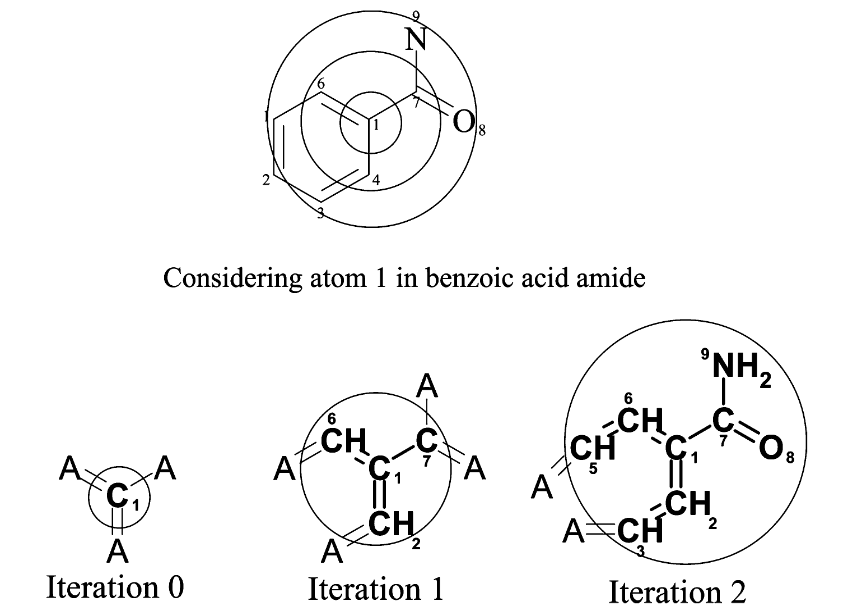
\includegraphics[width=0.5\textwidth]{iterative_updating.png}
	\caption{Illustration of the iterative updating in the computation of the ECFPs. In this example the atom type is used as an identifier. In iteration 0 the middle atom' identifier only represents the information about its own type. After the first iteration it has aggregated the information from its immediate neighbors and after the second iteration the represented substructure has grown even further. Reprinted from \cite{ECFP}. }
	\label{fig:iteration_ECFP}
\end{figure}

We clearly see ECFP's local nature. It manages to generate a global representation by using only local operations thereby implicitly encoding the molecule's structure. This is opposed to molecular descriptors discussed in the previous subsection that are based on global properties.

\begin{figure}[h]
	\centering 
	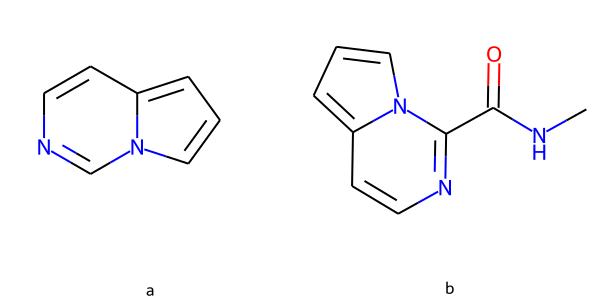
\includegraphics[width=0.5\textwidth]{test1.png}
	\caption{Molecular graphs corresponding to the SMILES strings `c1nccc2n1ccc2' and 1CNC(=O)c1nccc2cccn12'.}
	\label{fig:molsa}
\end{figure}
\begin{figure}[h]
	\centering 
	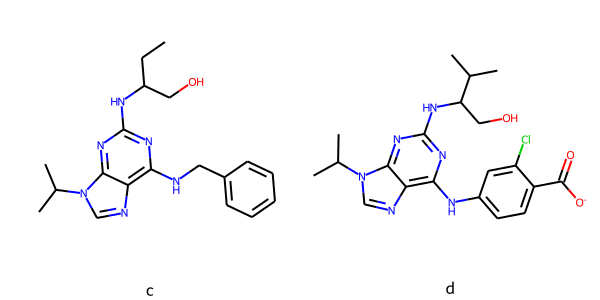
\includegraphics[width=0.5\textwidth]{test2.png}
	\caption{Molecular graphs corresponding to the SMILES strings `CCC(CO)Nc1nc(NCc2ccccc2)c2ncn(C(C)C)c2n1' and `CC(C)C(CO)Nc1nc(Nc2ccc(C(=O)[O-])c(Cl)c2)c2ncn(C(C)C)c2n1" }
	\label{fig:molsb}
\end{figure}
In the literature ECFP fingerprints are usually used with $n=2$ which is referred to as ECFP4 (4 being the maximum diameter of substructures considered). To understand the importance of this parameters,  we compare the predicted structural similarity of two pairs of molecules in Figure \ref{fig:molsa} and \ref{fig:molsb} for $n=1,2,3$. Furthermore, we list the similarity scores of Atom-Pair fingerprints \citep{atompairs} that are considered more suitable for representing larger molecules since they aggregate information of all pairs of atoms seperated by an arbitrary distance. The results are described in Table \ref{tab:dis_metric_2Dshapes}. The source code for this experiment can be found in the Appendix \ref{ch:a_sim}. We choose a pair of smaller molecules and one of larger molecules to understand if their size has any impact on the similarity scores. As expected, the predicted similarity drops for either pair with an increasing $n$ since larger and more dissimilar substructures are taken into account. However, the drop is substantially more significant for molecules a \& b.  This may be because for the first pair the proportion of dissimilar parts is larger for greater $n$ relative to the second pair. We remark that this hyperparameter appears to play an important role for when ECFPs are used as the input features for machine learning techniques. We can interpret $n$ as a regularisation parameter that penalises structurally too dissimilar molecules to be assigned too similar properties by a machine learning algorithm.
\begin{table}[h]
	\centering
	\begin{tabularx}{0.57\textwidth}{l
			r
			r 
			r
			r
		}
		\toprule
		& \multicolumn{3}{c}{Morgan Fingerprints} &   \\
		\cmidrule(r){2-4} 
		\bf{Molecules}  &  \multicolumn{1}{c}{\bf{ECFP2}}   & \multicolumn{1}{c}{\bf{ECFP4}}&  \multicolumn{1}{c}{\bf{ECFP6}} & \multicolumn{1}{c}{\bf{APFP}} \\
		\midrule
		a \& b   & 56.25\%   &  46.15\%  & 34.29\%    & 50.88\%   \\
		
		c \& d   & 68.66\%  &  58.71\% &  52.86\%  & 54.47\% \\
		
		
		\bottomrule
	\end{tabularx} 
	
	
	\caption{Sørensen-Dice similarity values \cite{sorensen1948method, dice1945measures} using different fingerprints for molecules in Figure \ref{fig:molsa} and Figure \ref{fig:molsb} respectively}
	\label{tab:dis_metric_2Dshapes}
\end{table}


Other circular fingerprints can be obtained by selecting different identifiers such as FCFPs (Functional Class Fingerprints) that is based on the pharmacophore role of the atoms in a molecule (\cite{ECFP}), SCFPs \citep{SCFP} or LCFPs \citep{LCFP}. The choice of the identifier is ultimately responsible for the discriminative abilities of the fingerprint. So expert knowledge is needed to make a meaningful decision.

As with numerical descriptors fingerprints are also a powerful mean to represent molecules in form of a fixed-size array. But a similar drawback as to numerical descriptors is that the best fingerprints depend strongly on the considered data set which again is  non-trivial to find.



\section{Learned Representations}
One of the major drawbacks of using molecular descriptors for drug design is that the performance of the method they are used for is dependent on an a priori selection of features and are therefore biased by expert knowledge \cite{merkwirth}. They are desined maunally. This means that a huge inductive bias is imposed and the resulting method can only perform as well as the feature selection allows. To remedy this problem an idea is to get away from these representations into a fixed predefined space but rather use machine or deep learning to learn the space itself. A particular method is the use of various kinds of Graph Neural Networks. Instead of just mapping the molecule to this fixed predefined representation Graph Neural Networks operate directly on the Graph and learn the features that are most suitable for the application. In this section we will first introduce Graph Neural Networks in their basic form as well as some extensions and then study the exact workflow in QSAR studies. Continuous degenerated representation due since the representation is encoded by differential mathematical operations and learned via backpropagation.

There are several anticipated benefits of using a learned representation \citep{SHEN201929}:
\begin{enumerate}
	\item It does not result in large, sparse representations as fingerprints.
	\item It provides a level of interpretability through \citep{duvenaud2015convolutional} (read)
	\item Attention algorithms can be adopted to f \citep{deepchemstable, graphattentionmpp}
	\item It could improce predictive performance on large data sets. \citep{yangMPP}
\end{enumerate}

\subsection{Molecular Graphs}
\label{sec:mol_graphs}
Molecular graphs are the entities that underlie most molecular notations. They are two dimensional objects that can be used to represent information about molecules. An example for a molecular graph is shown in Figure \ref{fig:mol_graph}. Vertices in the graph correspond to atoms in the molecule and edges represent bonds between them. We also note that the number of edges, i.e. the edge \emph{multiplicity}, may differ. This corresponds to the bond order in the molecule, i.e. the difference between the number of bonds and anti-bonds between two atoms, as introduced by \cite{pauling}. However, this graphical representation is not able to encode all information about its underlying molecule such as spatial information. Therefore, these need to encoded as features of the vertices and edges.

Formally a graph is defined as a tuple of sets $G = (V,E)$, where $V$ are the vertices of the graph and $E$ are the edges. Any edge $e \in E$ is uniquely identified by a pair of vertices $(v_1, v_2), \, v_1, v_2 \in V$ that it connects. In a molecular graph the vertices are given by the atoms and edges represent bonds between atoms. Compared to data structures like vectors, graphs are very high dimensional and irregular, simultaneously enabling the representation of more complex information and being harder to process.

In computers, graphs are represented by a matrix - most commonly by their adjacency matrix $A$. The entries of this matrix are given by 
\begin{equation}
A_{ij} = 
\begin{cases}
1 & \text{if there is an edge from } v_i \text{ to } v_j \\
0 & \text{otherwise.}
\end{cases}
\end{equation}
Note that for an undirected graph, like a molecular graph, the adjacency matrix is always symmetric. In order to represent a graph by its adjacency matrix, we need to make a non canonical choice of ordering the nodes. This is inconvenient for molecular graphs since these do not possess any kind of ordering and hence our representation is not well-defined. 

\begin{minipage}{0.5\textwidth}
	\centering
	\chemfig{OH\textsuperscript{1}-S\textsuperscript{2}(=[2]O\textsuperscript{3})(=[6]O\textsuperscript{4})-OH\textsuperscript{5}}
	\captionof{figure}{Molecular graph of sulfuric acid.}
	\label{fig:mol_graph}
\end{minipage}
\begin{minipage}{0.5\textwidth}
	\centering
	$
	\begin{blockarray}{cccccc}
	1 & 2 & 3 & 4 & 5 \\
	\begin{block}{(ccccc)c}
	0 & 1 & 0 & 0 & 0 & 1 \\
	1 & 0 & 1 & 1 & 1 & 2 \\
	0 & 1 & 0 & 0 & 0 & 3 \\
	0 & 1 & 0 & 0 & 0 & 4 \\
	0 & 1 & 0 & 0 & 0 & 5 \\
	\end{block}
	\end{blockarray}
	$
	\captionof{figure}{Adjacency matrix of the molecular graph representing sulfuric acid given the node ordering.}
	\label{fig:mol_adj_matrix}
\end{minipage}
\newline\newline
Figure \ref{fig:mol_adj_matrix} shows the adjacency matrix corresponding to the graph in Figure \ref{fig:mol_graph}. The ordering of the vertices is indicated by superscripts. If we assumed a different ordering of the vertices this would results in a permutation of the rows and columns of the adjacency matrix. As we will see, this is a common problem for Graph Neural Network which is attempted to be solve by the introduction of an \emph{inductive bias} devising algorithms that give the same results regardless of a permutation of the matrix.

In order to represent more information about the molecule the adjacency matrix is complemented with two more matrices - a node feature matrix and an edge feature matrix. The node feature matrix has the same number of rows as the adjacency matrix, where row $i$ corresponds to the feature values for node $i$. The number of columns may vary depending on the number of features that are chosen to be encoded. An example feature matrix is shown is Figure \ref{fig:mol_node_feature_matrix}. Finally, the edge feature matrix contains one row for every edge in the graph, where row $i$ corresponds to edge $i$ (TODO edge ordering?) and again the number of columns may vary depending on the number of features, see Figure \ref{fig:mol_edge_feature_matrix}.

\begin{minipage}{0.45\textwidth}
	\centering
	$
	\begin{blockarray}{ccccc}
	O & S & 0H & 1H  \\
	\begin{block}{(cccc)c}
	1 & 0 & 0 & 1 &  1 \\
	0 & 1 & 1 & 0 & 2 \\
	1 & 0 & 1 & 0 &  3 \\
	1 & 0 & 1 & 0 &  4 \\
	1 & 0 & 0 & 1 &  5 \\
	\end{block}
	\end{blockarray}
	$
	\captionof{figure}{Example feature matrix of the graph in Figrue \ref{fig:mol_graph}. The first two columns encode the atom type and the last two columns are a one-hot encoding of the number of implicit hydrogen atoms.}
	\label{fig:mol_node_feature_matrix}
\end{minipage}
\hfill
\begin{minipage}{0.45\textwidth}
	\vspace{.1cm}
	\centering
	$
	\begin{blockarray}{cccc}
	1 & 2 & 3  \\
	\begin{block}{(ccc)c}
	1 & 0 & 0 &  (1,2) \\
	0 & 1 & 0 &  (2,3) \\
	0 & 1 & 0 &  (2,4) \\
	1 & 0 & 0 &  (2,5) \\
	\end{block}
	\end{blockarray}
	$
	\captionof{figure}{Example edge feature matrix of the graph in Figure \ref{fig:mol_graph}. The choses features represent a one-hot encoding of the bond type.}
	\label{fig:mol_edge_feature_matrix}
\end{minipage}
\newline\newline
TODO : more sources on moelcular graphs 
While the graphical representation allows for the representation of complex 3D information of molecules, there are some drawbacks of working directly on the graph level. First, not all molecules can be represented as graphs \citep{molrep} such as those that contain bonds that cannot be explained by valence bond theory. Second, graphs are not a suitable means of depicting molecules whose arrangement of molecules change over time as this would require a reordering of the adjacency matrix every time. Finally, graphs are neither very compact nor easy to process. The adjacency matrix alone has a memory requirement quadratic in the number of atoms in the molecule and depending on the amount of atomic and bond information that is to be encoded the feature matrices might get even bigger. As opposed to this, a linear representation as a single string allows for using substantially less memory while being simultaneously easier to store and process by algorithms. Therefore, graphs are usually used as the basis of more compact representations that we are going to depict in the following subsections. 

\subsection{Graph Neural Networks}
\label{sec:GNN}

Convolutional Neural Networks (cite) have achieved remarkable success at learning representations of grid-like structures such as images. The idea to generalise these frameworks to less regular structures like graphs motivated the introduction of many Graph Convolutional Neural Networks (GCNNs) like in \citep{li2015gated,duvenaud2015convolutional,Kearnes_2016, Sch_tt_2017}. An attempt to unify all these approaches in a general framework was made by \cite{GilmerSRVD17} introducing Message Passing Neural Networks (MPNNs). In the following we will outline how MPNNs work and mention how they restore the previous approaches. 

MPNNs manage to represent properties of nodes and edges as well as structural knowledge about the graph. The properties are encoded in the node and edge feature matrices. Structural information is encoded implicitly via a similar aggregation step as for fingerprints in which a node receives knowledge about the neighbouring nodes and updates its own knowledge using that.

An entire forward pass of an MPNN can be divided into two phases: The message passing phase that runs for $T$ time steps and a consecutive readout phase. Each node stores information about its own features and those of its local environment in a hidden state vector ${\vecb h}_v^t \in {\mathbb{R}}^L$.  $\vecb h_v^0$ is initialised with the node's feature vector $\vecb x_v$. For each time step during the first phase any node receives `messages' about its neighbours' hidden states and then updates its own hidden state based on that. Specifically, this can be described as the two equations

\begin{eqnarray}
\vecb m_v^{t+1} & =& \sum_{w\in N(v)} M_t(\vecb h_v^t, \vecb h_w^t, \vecb e_{vw}) \label{eq:message_passing} \\
\vecb h_v^{t+1} & =& U_t(\vecb h_v^t, \vecb m_v^{t+1})\label{eq:updating}
\end{eqnarray}
where $\vecb m_v^t$ is the `message' node $v$ receives at time $t$ which is composed of the sum of the message functions $M_t$ from its immediate neighbours that can depend on their own hidden state $\vecb h_w^t$, the neighbour's hidden state $\vecb h_w^t$ and features of the edge connecting them.

After $T$ time steps, any node $v$ has now received information about any node $w$ that are at most $T$ edges away. This is because after the first step $w$'s neighbors receive information about $w$'s hidden state which is in turn incorporated in their own hidden state. In the next iteration, $w$'s neighbours pass their hidden state, incorporating information about $w$'s hidden state, to their own neighbours. This way, information about $w$'s hidden state is propagated through the graph and after $T$ iterations, $v$ receives this information.

The second readout phase now computes a feature vector for the whole graph as given in equation \ref{eq:readout}

\begin{equation}
	\hat{\vecb y} = R(\vecb h_1^T, \ldots, \vecb h_{|V|}^T) \label{eq:readout}
\end{equation}
Different choices for the functions $M_t, U_t$ and $R$ restore different Graph Neural Networks proposed in the literature. All of them have in common that they are differentiable and learned through backpropagation. Furthermore, $R$ must be permutation-invariant in order for the MPNN to be insensitive to the node ordering.
\begin{figure}[h]
	\centering 
	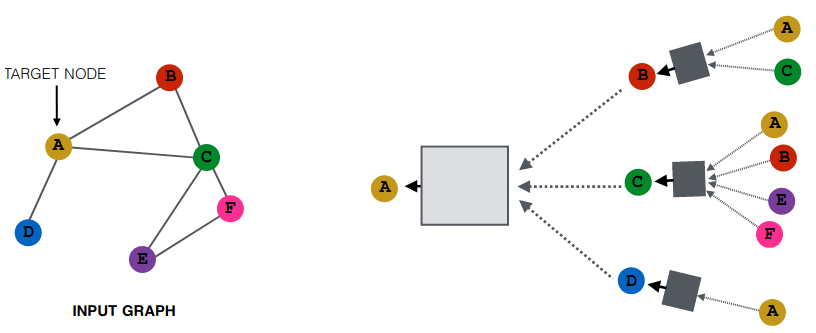
\includegraphics[width=0.7\textwidth]{MPNN.png}
	\caption{Illustration of the message passing in a MPNN. Reprinted from \cite{mpnn_graphics}. }
	\label{fig:mpnn}
\end{figure}
We illustrate how MPNNs recover two former architectures of Graph Neural Networks. For more detail, we refer to \cite{GilmerSRVD17}.

\subsubsection{Convolutional Neural Networks for Learning Molecular Fingerprints}
This archtiecture refers to the one porposed by \cite{duvenaud2015convolutional}. Here, the message function $M_t$ is the same across all time steps and given by
\begin{align*}
M(\vecb h_v, \vecb h_w, \vecb e_{vw}) &= (\vecb h_w, \vecb e_{vw}), 
\intertext{where $(\cdot, \cdot)$ denotes concatentation. The update and readout functions are given by}
U_t(\vecb h_v^t, \vecb m_v^{t+1}) & = \sigma(\vecb H_t^{\text{deg}(v)} \vecb m_v^{t+1})
\intertext{which includes learnable parameters as given by the matrices $\vecb H_t^{k}$ for all time steps $t$ and node degrees $k$. $\sigma$ denotes the sigmoid activation function. Finally, the readout function is given by}
 R(\vecb h_1^T, \ldots, \vecb h_{|V|}^T) &= f\left(\sum_{v,t} \text{softmax}(\vecb W_t \vecb h_v^t)\right)
\end{align*}
with learnable matrices $\vecb W_t$ for all time steps $t$ and a neural network $f$. 
\begin{comment}
\subsubsection{Deep Tensor Neural Networks}
This archtiecture refers to the one porposed by \cite{Sch_tt_2017}. Here, the message function at time $t$ is given by 
\begin{align*}
M_t(\vecb h_v, \vecb h_w, \vecb e_{vw}) &= \tanh\left(\vecb W^{fc}((\vecb W^{cf} \vecb h_w^t + \vecb b_1)\odot (\vecb W^{df} \vecb e_{vw} + \vecb b_2 ))\right), 
\intertext{where $\odot$ denotes the element-wise product, $\vecb W^{fc},\vecb W^{cf}, \vecb W^{df}$ are learnable matrices and $\vecb b_1, \vecb b_2$ are learnable biases. The update function at time $t$ is given by:}
U_t(\vecb h_v^t, \vecb m_v^{t+1}) & = \vecb h_v^t \ \vecb m_v^{t+1}
\intertext{Finally, the readout passes each final hidden state individually through a single hidden layer neural netork and sums the results:}
R(\vecb h_1^T, \ldots, \vecb h_{|V|}^T) &=\sum_v \text{NN}(\vecb h_v^t)
\end{align*}
\end{comment}
\subsection{Directed MPP ? \cite{yangMPP}}
\subsubsection{Graph Convolutional Neural Networks}
\label{sec:GCN}
These belong to the most popular classes of Graph Neural Networks and was proposed by \citep{gcn}. A detailed derivation of the message and update functions can be found on \cite{GilmerSRVD17}. The resulting functions are given by:

\begin{align*}
M_t(\vecb h_v^{t}, \vecb h_w^{t}) &= \sum_{w \in N(v) \cup \{v\}}(\deg(v)\deg(w))^{-1/2} \vecb h_w^t
\intertext{The update function at time $t$ is given by:}
U_t(\vecb h_v^t, \vecb m_v^{t+1}) & = \sigma (\vecb W^t \vecb m^{t+1})
\end{align*}
with a trainable matrix $\vecb W^t$ and a non-linear activation function $\sigma$, e.g. ReLU. This can be thought of as a generalisation of the MPNN framework that includes self-loops in the message passing step.

\subsubsection{Graph Attention Networks}
Graph Attention Networks proposed by \cite{gan} extend GCNs by replacing the normalisation constants $\deg(v)\deg(w)$ in the aggregation step by a learned attention score
\begin{align*}
M_t(\vecb h_v^{t}, \vecb h_w^{t}) &= \sum_{w \in N(v)}\alpha^t_{vw} \vecb h_w^t.
\end{align*}
The attention score weighes the information from neighbours according to how important they are. Details about how $\alpha_{vw}^t$ is computed can be retrieved from the paper \citep{gan}.
\subsubsection{Attentive FP}
The most recent state of the art Graph Neural Network architecture was propsed by \cite{attentivefp}. It proceeds similarly to GANs by stacking multiple attention layers together with Gated Recurrent Units (GRUs) to update the nodes' hidden states recursively and allow an atom to focus on its most important neighbors. To generate the final graph embedding, Attentive FP treats the whole molecule as a virtual node that connects to all its atoms. Then, it employs the same architecture as for the individual atoms to learn the molecule's final representation. 
These 
GCN, GAN, Attentive FP?


\subsection{Sequence modeling}
SMILES RNNs, LSTMs? \cite{honda}
\section{Case study}


As an example for a full MPP workflow, we choose \cite{STOKES2020688} who used a Graph Neural Network to predict the growth of E. Coli. Their approach can be divided into three stages. The fist stage concerns the training of the model and a classifier according to Figure \ref{fig:mpp_workflow}. The molecular representation was built using a directed-message passing neural network \cite{yangMPP} and can therefore be classified as a learned representation. Similarly to ECFP fingerprints, (D-)MPNNs can struggle to represent global features of molecules, especially if the number of message passing iterations is greater than the longest path in the molecule as discussed in section \ref{sec:GNN}. Therefore, the final representation generated by the D-MPNN was augmented with 300 additional molecule-level features. This combined representation was then input in a feed-forward neural network that outputs a number between 0 and 1 as the prediction of the molecule showing growth inhibitory against E. Coli. This whole architecture is trained in an end-to-end fashion such that the D-MPNN can generate a representation that is highly attuned to the desired property.
The training of this architecture was performed using a set of 2335 molecules that had been classified as hit or non-hit using 80 \% growth inhibition against E. coli BW251113 \cite{ZAMPIERI20171214} as a hit cut-off. On the test data this model achieved an AUC-ROC score of 0.896.

In the secong stage, 20 folds of the trained model using different weight initialisations were applied to 6,111 molecules from the Drug Repurposing Hub \citep{corsello} to predict their probability of growth inhibition against E. Coli. The 20 different results were averaged to arrive at the final prediction scores. 

Finally, the best scoring 99 molecules were empirically tested for growth inhibition out of which 51 displayed this property. The resulting 51 molecules were ranked according to their clinical phase of investigation, structural similarity to the training data set and their toxicity that was also predicted using a D-MPNN. This resulted in the discovery ot the broad-spectrum bactericidal antibiotic halicin with a very low structural similarity to its nearest neighbour antibiotic in the training data emphasising the model's capacity to generalise. 

This case study shows the versatility and potential of using Graph Neural Network for property prediction in early drug discovery. They could be employed for both prediction of growth inhibitory effects as well as toxicity and resulted in the finding of a new antibiotic after years of stagnation in this field. \cite{STOKES2020688} also reported the prediction scores using Morgan fingerprints and various classifier and the rank of the newly discovered antibiotic halicin was lower in all of them ranging between 773-2644 compared to 69 for the D-MPNN approach. Therefore, it could be argued that halcin would not have been found if molecular fingerprints had been used. However, between there is still some correlation among the top scoring molecules. For instance, both the D-MPNN and Morgan fingerprints predict the same highest ranking molecule and the fourth place for D-MPNN is in second place for Morgan fingerprints. The question that remains to be answered is if this is just a correlation of numerical values and halicin being ranked much higher for learned representations is just a fortunate coincidence or if the predictions of GNNs actually carry more physical relevance.

Despite this breakthrough using the GNN approach, \cite{STOKES2020688} still emphasise the importance of a combination of \emph{in silico} and empirical investigations. 


ADMET study, other properties?
\subsection{De novo design}

\section{Discussion}
Artificial intelligence and machine learning are currently one of the most rapidly evolving research areas and the progress in these fields has direct impacts on  a great variety of disciplines. In particular, we have hinted at ther potential to revolutionise the entire field of drug discovery coming with significant reductions in time and resources (TODO where? maybe time span to see how little time). Most recently, a variety of Graph Neural Networks has been introduced as a way to automatize the feature selection for molecular property prediction. Instead of relying on expert knowledge to select the most relevant attributes to be used for a computer-interpretable interpretation, which has been shown to heavily impact the performance of the property prediction \citep{tian}, Graph Neural Network manage to learn a continuous vector representation that is highly attuned to the property of concern. 

While many studies report that learned representations are superior to fixed representations in term of the property prediction accuracy for a variety of different applications \citep{wu2018moleculenet,yangMPP, korolev}, there is still no consensus on this and others report the dominance of descriptor-based approaches and fingerprints \citep{mayr, jiang}. This suggests that there are other relevant factors that influence which approach is better. Since there a substantially more parameters involved in learning a representation compared with using a fixed representation a sufficiently large data set is critical to learned approaches. Something else to take into account is the mode of evaluation. As mentioned by \cite{SHEN201929}, the evaluation of model performance is critical to molecular property prediction. This is because unlike images there is no standard to generating ground truth labels for the data. These are usually obtained from experiments and experimental procedures can differ and are subject to human errors. Furthermore, baseline models are often not tuned enough to reach peak performance.( Finally a fundamental assumption of employing and comparing machine different machine learning models is that training and test data are all independently identically distributed. It has been noted that for different molecules this requirement is very hard to verify let alone achieve.) (find source)
 

In terms of the required computational resources, fixed representations can be computed much quicker than learned approaches


The last aspect to take into consideration is interpretability. Graph Neural Networks like all deep learning algorithms work as a black box. There is no real way to assign any meaning to its final representation in terms of interpreatblity.  For descriptor based models on the other hand the SHAP method \citep{lundberg2017unified} allows for a way to interpret the final prediction scores by computing the contribution of each input feature that had been selected. Therefore, it enables an understanding of which features turned  out to be the most relevant for a particular property. 

I personally think that the future of property prediction is within learned molecular representations. While their lack of interpretability is a considerable drawback, there are two major advantages. First, GNNs are able to achieve state-of-the-art performance and they have already successfully used to impel (word?) areas that were stagnating before their introduction \citep{STOKES2020688}. While there are still publications reporting better results for descriptor-based approaches, GNN's great potential to be adjusted will probably keep improving their results (phrasing). For example, since the message passing approach may struggle to represent global properties of a graph, a global readout (cite) has been proposed helping overcome this. Secondly, GNNs enable their application to property prediction without having to rely on domain experts that need to select appropriate features. This allows for a wider application across disciplines making GNNs a versatile and promising tool for the future.
\section{Conclusion}
In this report we have studied fixed and learned molecular representations for molecular property prediction. Two classes of learned representations were introduced, namely descriptor-based approaches and molecular fingerprints. We compared atom-pair descriptors with the most popular Morgan fingerprints to understand hoe they capture similarities between different molecules. We found that ....
After that, we introduced molecular graphs and Graph Neural Networks that operate directly on the graph level as an example for a learned representation. Recent advancements for GNNs were outlined with the general message passing framework and more recent improvements through D-MPNNs, Graph Attention Networks and Attentive FP. These highlight the capability of further improvements for GNNs and henceforth their potential in molecular property prediction. Finally, we compared learned representations with fixed representations in terms of accuracy, computational costs and interpretability. Despite fixed approaches being better in terms of the two latter aspects, we hypothesised Graph Neural Networks to be the future molecular prpoerty predictions. On the one hand this was because of their state-of-the-art performance that is probable to be improveed further due to their flexibility to be extended (wphrasing) and on the other hand due to their wide applicability given that they do not require expert knowledge to be used. 